% =====================================================================================
% DEDV_2_revised.tex -- revised version of DEDV_2.tex (the faithful transcription).
% Every change, with its section and reason, is listed in REPORT_CHANGES.md.
% Values that could not be verified against CONTEXT_PROMPT.md, the code or bench/results are
% marked with "% VERIFY:" comments.
% Build: pdflatex DEDV_2_revised && bibtex DEDV_2_revised && pdflatex DEDV_2_revised (x2)
% =====================================================================================
\documentclass[pdflatex,sn-mathphys-num]{sn-jnl}

\usepackage{graphicx}%
\usepackage{multirow}%
\usepackage{amsmath,amssymb,amsfonts}%
\usepackage{xcolor}%
\usepackage{textcomp}%
\usepackage{booktabs}%
\usepackage{array}%
\usepackage{tikz}%
\usetikzlibrary{positioning,arrows.meta,fit}%
\usepackage{pgfplots}%
\pgfplotsset{compat=1.18}%
\usepgfplotslibrary{colorbrewer}%

\graphicspath{{../bench/results/}}
\newcommand{\code}[1]{\texttt{#1}}

\raggedbottom

\begin{document}

\title[DEDV]{DEDV - A Dynamic Encryption Digital Vault for a secured document storage}

\author[1]{\fnm{K.T.} \sur{Hiranmayi}}\email{hiranmayi.23bcb7022@vitapstudent.ac.in}
\author*[1]{\fnm{Ngangbam} \sur{Indrason}}\email{indrason.n@vitap.ac.in}
\author[1]{\sur{Soumya}}\email{soumya.23bcb7020@vitapstudent.ac.in}
\author[1]{\sur{Swapnil}}\email{swapnil.23bcb7031@vitapstudent.ac.in}
\author[1]{\fnm{Pallam} \sur{Sneitha}}\email{snehita.23bcb7237@vitapstudent.ac.in}

\affil*[1]{\orgdiv{School of Computer Science and Engineering}, \orgname{VIT-AP University},
\orgaddress{\city{Amaravati}, \postcode{522241}, \state{Andhra Pradesh}, \country{India}}}

\abstract{Conventional document storage applies the same protection to every document, although
documents differ in their security requirements. This paper presents the Dynamic Encryption
Digital Vault (DEDV), a document vault that predicts a security level from document and
usage-context attributes and encrypts each document with the algorithm mapped to that level. Five
machine learning models, K-Nearest Neighbors (KNN), Decision Tree (DT), XGBoost (XGB), Multinomial
Logistic Regression (MLR) and Random Forest (RF), were evaluated on experimental survey data
comprising 402 records from 67 respondents. Random Forest achieved a macro-F1 score of
0.389~$\pm$~0.026 using ten input features. A reduced seven-input configuration achieved
0.380~$\pm$~0.024 and was selected using predefined criteria that balance input reduction,
classification performance and under-classification risk. The prototype is a Windows desktop
application. It derives a key-encryption key from the vault password with Argon2id, seals a
separate key for every file under a vault master key, refers to each file key by a random token
kept in a separate key store, releases a key only to an unlocked session, and records every key
release in a hash-chained audit log. The user may raise the predicted level but not lower it.
On the test machine, storing a 1~MB file took about 6--8~ms and reading it about 12~ms at four of
the five levels; the Enhanced level took 0.3--0.8~s per file because it generates and loads an
RSA-4096 key pair for every file, and unlocking the vault took 0.41~s.
The Enhanced class contains only eight records, so its predictions are not reliable. Further
research should expand the dataset, validate the model on more representative data and evaluate
the system with real-world documents and users.}

\keywords{Dynamic encryption, Digital vault, Security level classification, Random Forest, Key
management}

\maketitle

\section{Introduction}\label{sec1}

Cloud platforms and digital libraries are preferred for data storage instead of storing the data
exclusively locally \cite{asim2026adoption}. This makes it easy to use and access the data but
also creates the concern of security and protection of the data.

Encrypting each file with the highest security seems good but results in more storage and time
consumption. Thus the required protection for data or a document depends on various factors
including circumstances in which it will be used. A document containing normal data may not
require the same level of protection as one containing confidential business information or a
document containing personal information. Using the same protection method for all the data being
stored won't account for these differences. The level of protection a document needs will depend
on various factors including document sensitivity, file type, content classification, ownership,
user role, sharing requirements, access frequency, and the risk associated with unauthorized
access \cite{khan2023cybersecure,smallwood2012safeguarding,phoha2014context}. Access requirements
from multiple devices and retention can also affect the level of protection required for the
document. Hence, the context of usage and the features of the document must be considered while
implementing protection protocols.

Encryption is necessary while protecting the data and choosing the type of encryption algorithm
is a part of implementing the security \cite{akinkunmi2024importance}. The storage system must
also maintain the encryption along with keys and user access to the data in the storage. When an
authorized user is accessing the data it is necessary to retrieve the decryption key for user
access. These operations should work together for consistent document protection during storage
and retrieval.

Previous papers dealt with cloud storage, data classification, machine learning models and
encryption algorithms for secure data storage in digital and cloud models. The
Confidentiality-based Data Classification-as-a-Service (C2aaS) approach emphasises how data can be
classified based on confidentiality requirements and how the classification can help with the
encryption decision in cloud environments: the level of protection is classified based on the
confidentiality requirement of the data rather than using the same level of security for every
item \cite{ali2023confidentiality}. Jabbar and Bhaya proposed a private cloud security approach
that deals with machine learning, data classification and cryptographic methods. Network attack
detection along with user data classification based on importance and application of different
encryption algorithms is considered in their work \cite{jabbar2022secure}. This provides a related
example of a machine learning model that supports differentiated data protection. Another model
deals with the classification of cloud data to enhance security by adding data characteristics and
security requirements when selecting the type of encryption required
\cite{singh2018classification}. The broader relevance to this work is that classification can
provide a basis for implementing an appropriate protection mechanism based on the requirements of
the data being stored. Machine learning has also been applied to cloud encryption and retrieval.
Malhotra and Singh researched a keyword-ranking approach using an artificial neural network for
encrypted data. Their work considers the usage of machine learning in encryption and retrieval
rather than just using it for general data classification \cite{malhotra2023efficacy}.
Confidential machine learning deals with another aspect of this problem: the platforms that train
models on sensitive information may not be fully trusted. Techniques used in this approach include
homomorphic encryption, hybrid cryptographic protocols, garbled circuits, perturbation-based
methods and hardware-assisted approaches. These techniques have a trade-off between
confidentiality, computational cost and model utility \cite{sagar2021confidential}. Together these
studies provide different backgrounds for various components. Their approaches are different and
they focus on different security objectives.

The reviewed studies establish that data classification, machine learning, encryption, and
cryptographic protection have already been explored in cloud-security research
\cite{thabit2023data}. The research gap here should therefore not be framed as the absence of
machine learning or encryption in existing systems. Instead, the gap concerns the particular
combination being investigated. We consider document characteristics alongside user and
usage-context parameters when predicting the required security level. It defines separate personal
and enterprise security hierarchies, evaluates candidate machine-learning models for the
prediction task, and links the resulting classification to an encryption configuration. The
framework also incorporates tokenized key management into the document-protection workflow. The
token provides a reference for locating the key associated with an encrypted document during an
authorized retrieval operation. This brings security-level assignment, encryption configuration
selection, and key association into one digital-vault design. The contribution should be
described in terms of this integration and its evaluation. It should not imply that the
individual machine-learning models, encryption techniques, or token-based references are new
inventions.

The Dynamic Encryption Digital Vault (DEDV) is designed as a framework for document storage that
connects the level of security, predicted by a machine learning model, with the encryption of the
document. For user access a controlled document retrieval system is implemented. The main idea is
to determine the required level of protection for a document based on available parameters of the
document and contextual data \cite{sasikumar2025enhancing}.

The main contributions of the proposed work can be presented as follows:
\begin{itemize}
\item Context-based security-level prediction: The framework uses document-related and contextual
parameters to determine the security level assigned to a document.
\item Separate personal and enterprise hierarchies: DEDV provides two environments for document
storage: a personal vault with three levels of security and an enterprise vault with five levels
of security.
\item Comparative evaluation of machine learning models: Five models, KNN, RF, XGB, MLR and DT, are
evaluated for security level prediction, with the final model being RF based on the experimental
results.
\item Security level to encryption mapping: The predicted level is mapped to the associated
encryption algorithm (Table~\ref{tab4}).
\item Tokenized key-management workflow: The framework separates encryption keys from encrypted
documents and uses tokenized references to support key retrieval during authorized decryption.
\item Working prototype and measurements: a desktop implementation with a password-based key
hierarchy, a token-indexed key store, audited key release and an upward-only override of the
prediction, together with benchmarks of every security level (Sections~\ref{sec6}
and~\ref{sec8}).
\end{itemize}

DEDV addresses how document attributes and usage-context information can be considered while
assigning a security level, mapping it to an encryption algorithm and managing the keys.

DEDV proposes two security hierarchies. The personal vault consists of three security levels and
the enterprise vault consists of five security levels, with an option to choose between two
encryptions for the highest predicted class. The system uses a mapping between each security level
and its corresponding encryption algorithm. This framework allows two different environments
within a single application.

The design considered parameters such as document sensitivity, file type, file size, content
classification, user role, organization type, ownership, access frequency, sharing requirements,
risk level, multiple-device access and retention period. These characteristics cover various
aspects of a document and its intended use. The survey captured ten of them as inputs, and the
final model uses seven (Section~\ref{sec5-1}).

Five machine learning models are considered for the prediction task: K-Nearest Neighbors (KNN),
Random Forest (RF), XGBoost (XGB), Multinomial Logistic Regression (MLR), and Decision Tree (DT).
These models are compared using experimental data and the final decision engine is determined by
the observed evaluation results.

DEDV also implements encryption key separation and tokenized key management. Each file key is
stored, sealed under a vault master key, in a separate key database, and a random token serves as
the reference to it. When a document is opened, the system first checks that the vault is unlocked
and that the token belongs to the requested file before it releases the key, and it records every
such request.

DEDV connects four related operations: determining the security level, selecting the mapped
encryption algorithm, managing the encryption key and controlling the retrieval process.

This paper is organized as follows. Section~\ref{sec2} discusses related works. The motivation of
this work is laid down in Section~\ref{sec3}. The proposed system model is discussed in
Section~\ref{sec4}. Section~\ref{sec5} describes the methodology. Section~\ref{sec6} describes the
implementation. The experimentation is shown in Section~\ref{sec7}, and its results are discussed
in Section~\ref{sec8}. Section~\ref{sec9} deals with the limitations of the proposed work. The
future scope of work is discussed in Section~\ref{sec10} and Section~\ref{sec11} concludes the
paper.

\section{Related Works}\label{sec2}

Research on protected digital storage has explored machine learning, data classification,
cloud-based encryption and cryptographic techniques. The aim of these studies is to protect data
while considering factors like confidentiality, computational overhead and the efficiency of data
storage and retrieval. The following works are relevant to the development of the Dynamic
Encryption Digital Vault (DEDV).

\subsection{Confidentiality-Based Data Classification-as-a-Service (C2aaS)}

Ali et al. \cite{ali2023confidentiality} proposed Confidentiality-based Data
Classification-as-a-Service (C2aaS) to address the security and processing overhead associated
with cloud data storage. The authors of this paper focus on confidentiality risks created by
storing data in plaintext and how encrypting the data can increase processing requirements. Their
proposed model classifies data according to security level and processes it dynamically before
cloud storage. The objective is to secure confidential data while reducing unnecessary system
overhead. C2aaS is closely related to DEDV because both approaches use security classification to
determine how data should be handled. However, DEDV focuses on a digital-vault framework in which
document characteristics and usage-context parameters contribute to a predicted security level.
It also defines separate security hierarchies for personal and enterprise environments and
connects the predicted level to an encryption configuration and tokenized key-management
workflow.

\subsection{Security of Private Cloud using ML and Cryptography}

Jabbar and Bhaya proposed a security model for private cloud environments that combines network
attack detection with data classification and encryption. Their approach has two phases. In the
first phase normal and abnormal traffic is detected whereas the second classifies the user data
according to its importance and applies different encryption algorithms. The authors evaluate
machine learning algorithms for attack detection and data classification, including Random
Forest, Decision Tree, Logistic Regression, and Stochastic Gradient Descent
\cite{jabbar2022secure}. This work demonstrates how machine learning can support different
security operations in a cloud environment. Its approach is relevant to DEDV because it links data
classification with the selection of encryption methods. DEDV focuses on predicting the required
security level of an individual document using a comparison of five models. The selected model is
then used as the decision engine within the vault's personal or enterprise security hierarchy.

\subsection{Classification of Data to Enhance Data Security in Cloud Computing}

The study Classification of Data to Enhance Data Security in Cloud Computing examines how data
classification can support the selection of suitable encryption methods in cloud environments.
The authors explain that data security requirements vary according to the type of information and
the requirements of its owner. Their work proposes classifying cloud data using relevant security
parameters so that an appropriate encryption method can be selected dynamically
\cite{singh2018classification}. This study supports the principle that different data items may
require different levels of protection. It focuses on the relationship between encryption and
classification efficiency. DEDV builds on this general principle by considering a combination of
document, user, and usage-context parameters in its security-level decision process. It also
distinguishes personal and enterprise storage requirements rather than using a single hierarchy
for both environments.

\subsection{An Efficacy Analysis of Data Encryption Architecture for Cloud Platform}

The authors of An Efficacy Analysis of Data Encryption Architecture for Cloud Platform propose a
machine-learning-based model for cloud data encryption and retrieval. This model combines
Symmetric Searchable Encryption with a keyword ranking method based on Artificial Neural Network
(ANN). The study compares the proposed model with multiclass Support Vector Machine (SVM) and
Na\"{\i}ve Bayes approaches and evaluates its operational performance using measures that include
the true-positive rate and false-positive rate \cite{malhotra2023efficacy}. This work is relevant
because it applies machine learning within a cloud encryption and retrieval architecture. It shows
that machine learning can contribute to security-related operations beyond conventional data
classification. DEDV focuses on predicting a document's required security level and uses that
prediction to select the mapped encryption algorithm. The five candidate models in DEDV are
evaluated for this security-level prediction task.

\subsection{Confidential Machine Learning on Untrusted Platforms: A Survey}

Sharma and Chen presented a survey of confidential machine learning on untrusted platforms,
including public cloud and edge environments. This study focuses on machine learning and
cryptographic approaches for protecting sensitive training data during outsourced computation,
namely hybrid cryptographic protocols, homomorphic encryption, garbled circuits,
perturbation-based methods and hardware-assisted approaches. The authors examined the trade-off
between model utility, confidentiality and computational cost
\cite{asikis2020optimization,sagar2021confidential}. This survey provides a broader security
perspective for systems that combine machine learning with outsourced computing
\cite{jauernig2020trusted}. It is relevant to DEDV because a secure vault must consider not only
how a document is encrypted but also how sensitive information and associated operations are
protected. The survey focuses on confidential machine learning rather than a vault for documents
that predicts security levels, maps them to encryption configurations and manages document access
through tokenized key references.

\subsection{Comparative Analysis of Existing Work}

Table~\ref{tab1} presents a comparison of the reviewed studies, highlighting their main focus,
relevant contributions, and relationship to the proposed DEDV system.

The reviewed studies establish that data classification, machine learning, encryption, and
cryptographic protection have already been explored in cloud-security research. Therefore, the
motivation for DEDV is not simply to combine machine learning with encryption, since previous
work has already investigated related combinations.

\begin{table}[h]
\caption{Comparison of Existing Studies with the Proposed DEDV}\label{tab1}
\begin{tabular}{@{}cp{3cm}p{3.6cm}p{3.6cm}@{}}
\toprule
Reference & Main Focus & Relevant Contribution & Relationship to DEDV \\
\midrule
\cite{ali2023confidentiality} & Confidentiality-based data classification for cloud storage &
  Dynamically handles data according to its security level & Supports security-level-based data
  handling \\
\cite{jabbar2022secure} & Private-cloud security using machine learning and cryptography &
  Combines attack detection, data classification, and encryption & Demonstrates ML-based
  classification linked to encryption \\
\cite{singh2018classification} & Data classification for cloud security & Uses data
  classification to guide encryption selection & Supports differentiated protection based on
  data requirements \\
\cite{malhotra2023efficacy} & Machine-learning-based cloud encryption and retrieval & Combines
  searchable encryption with ANN-based keyword ranking & Demonstrates ML integration within an
  encryption and retrieval architecture \\
\cite{sagar2021confidential} & Confidential machine learning on untrusted platforms & Surveys
  cryptographic and other techniques for protecting ML computations & Provides background on
  confidentiality and cryptographic protection \\
\botrule
\end{tabular}
\end{table}

\subsection{Research Gap}

The proposed work therefore focuses on integrating these capabilities within a single
digital-vault framework. DEDV considers document characteristics together with user and
usage-context parameters to predict the required security level. It defines three levels for the
personal vault and five levels for the enterprise vault, evaluates five candidate machine learning
models for the prediction task, and uses the selected model to determine the corresponding
encryption configuration. The framework also includes tokenized key management to support
controlled key association and retrieval during authorized decryption.

Based on the five studies reviewed here, this particular combination of context-based
security-level prediction, separate personal and enterprise hierarchies, encryption-configuration
selection, and tokenized key management provides the direction for DEDV. The contribution lies in
the integration and evaluation of these components, rather than in claiming that each component is
individually new.

\section{Motivation}\label{sec3}

\subsection{Motivation}

Existing works have explored machine learning, classification and encryption to improve the
security of data. The protection required depends on factors other than content: sensitivity,
exposure consequences, access requirements and the duration of protection also affect the
security level needed. DEDV considers these factors while assigning security levels to stored
documents.

The proposed model also considers contextual parameters to predict the security level required
for the document. The personal vault environment has three security levels and the enterprise
vault has five, with a choice between two encryption algorithms for the highest predicted class.
This allows the protection level to follow the required environment rather than using the same
hierarchy for every document.

DEDV is tested using five machine learning models: K-Nearest Neighbors (KNN), Random Forest (RF),
XGBoost (XGB), Multinomial Logistic Regression (MLR), and Decision Tree (DT). Random Forest is used
as the decision engine based on the model selection process \cite{speiser2019comparison}. Its
purpose is to take the input parameters and predict a security level, which is then mapped to the
corresponding encryption configuration.

Tokenized key management is also incorporated in the framework. Encrypted documents and encryption
keys are stored separately and tokens provide a reference to the associated decryption keys.
During document retrieval, authorization is confirmed before decryption. This forms the connection
between security level prediction, encryption and controlled document access.

\subsection{Challenges}

Selecting parameters that provide useful information for security level prediction is one of the
challenges in DEDV. The Random Forest model uses seven input parameters: Sensitivity, Who Should
Access, Access Frequency, Exposure Consequence, Protection Duration, Multiple Devices and Multiple
Locations/Countries. These inputs consider different aspects of document sensitivity and the
context of usage, and their representation must remain the same between training and prediction.

Mapping the predicted security level to the corresponding encryption configuration is another
challenge. The system considers the vault type, as personal and enterprise vaults have different
sets of security levels. An incorrect mapping might result in an encryption that does not match
the assigned level.

The encryption key and encrypted document are maintained separately, so key management introduces
another challenge. The system must preserve the association between the document, its token and
the corresponding key. During decryption and retrieval, authorization must be verified before the
key is released. To maintain the intended document protection workflow it is necessary to
maintain this association and to restrict key access.

\section{Proposed System Model}\label{sec4}

Fig.~\ref{fig1} illustrates the system model of the Dynamic Encryption Digital Vault (DEDV) as it
is implemented, from contextual security-level prediction to vault-specific encryption, separate
key management, and authorized document retrieval. The required security level is predicted from
contextual and document-related parameters. The machine learning model used for decision making
is a Random Forest. It takes seven inputs and classifies the document into one of four security
classes: Low, Standard, Enhanced and High/Critical \cite{phoha2014context}. Together with the class
it reports a confidence, the probability of the predicted class.

The vault environment decides which final levels are allowed. The enterprise vault contains five
security levels and the personal vault contains three. A Low, Standard or Enhanced prediction
becomes the final level directly. For a High/Critical prediction an enterprise user chooses High
or Critical; a personal vault offers neither, so no level is assigned and the user is told to use
an enterprise vault. The system maps each final level to an encryption algorithm
(Table~\ref{tab4}) \cite{sasikumar2025enhancing}. It predicts a security level and never assigns
an algorithm directly.

\begin{figure}[h]
\centering
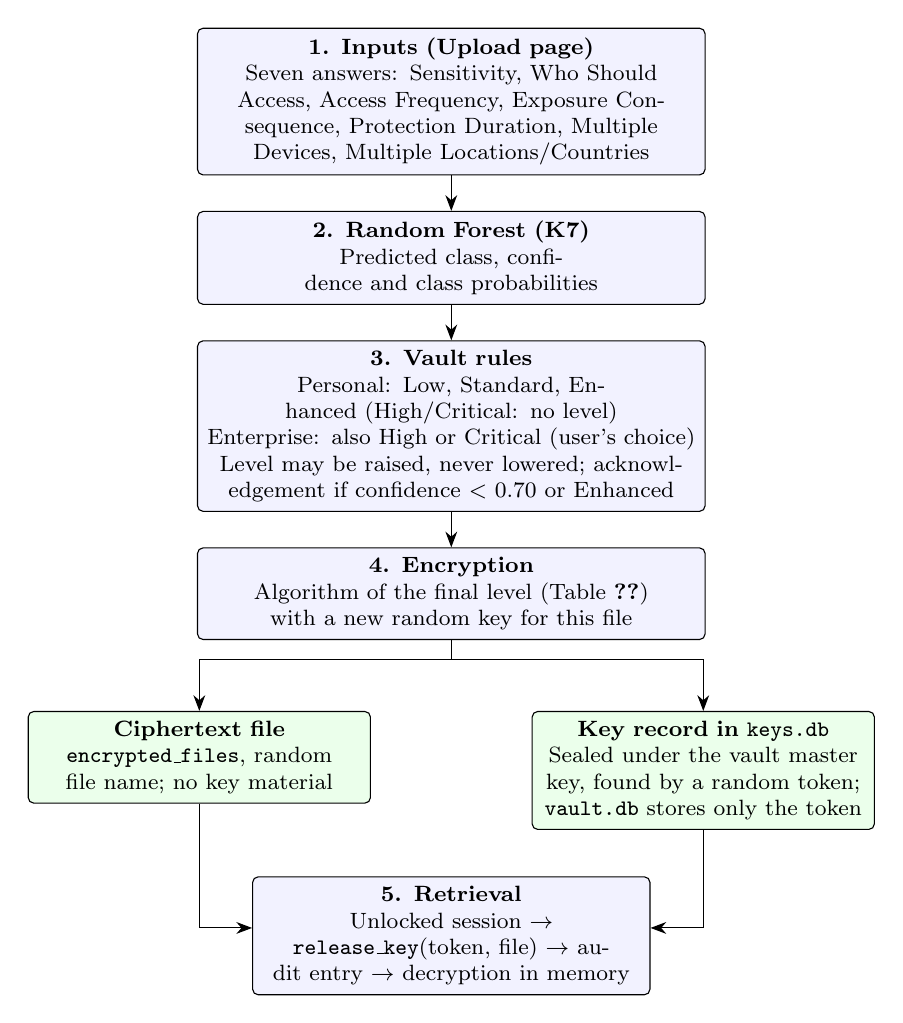
\begin{tikzpicture}[
  box/.style={draw, fill=blue!5, rounded corners=2pt, align=center, text width=6.2cm,
              font=\footnotesize, inner sep=3.5pt},
  side/.style={draw, fill=green!8, rounded corners=2pt, align=center, text width=4.1cm,
               font=\footnotesize, inner sep=3.5pt},
  arr/.style={-{Stealth[length=2mm]}},
  node distance=4.5mm]
\node[box] (b1) {\textbf{1. Inputs (Upload page)}\\ Seven answers: Sensitivity, Who Should
  Access, Access Frequency, Exposure Consequence, Protection Duration, Multiple Devices, Multiple
  Locations/Countries};
\node[box, below=of b1] (b2) {\textbf{2. Random Forest (K7)}\\ Predicted class, confidence and
  class probabilities};
\node[box, below=of b2] (b3) {\textbf{3. Vault rules}\\ Personal: Low, Standard, Enhanced
  (High/Critical: no level)\\ Enterprise: also High or Critical (user's choice)\\ Level may be
  raised, never lowered; acknowledgement if confidence $<$ 0.70 or Enhanced};
\node[box, below=of b3] (b4) {\textbf{4. Encryption}\\ Algorithm of the final level
  (Table~\ref{tab4}) with a new random key for this file};
\node[side, below=9mm of b4, xshift=-3.2cm] (enc) {\textbf{Ciphertext file}\\
  \code{encrypted\_files}, random file name; no key material};
\node[side, below=9mm of b4, xshift=3.2cm] (km) {\textbf{Key record in \code{keys.db}}\\ Sealed
  under the vault master key, found by a random token; \code{vault.db} stores only the token};
\node[box, below=30mm of b4, text width=4.8cm] (b6) {\textbf{5. Retrieval}\\ Unlocked session $\rightarrow$
  \code{release\_key}(token, file) $\rightarrow$ audit entry $\rightarrow$ decryption in
  memory};
\foreach \a/\b in {b1/b2, b2/b3, b3/b4}
  \draw[arr] (\a) -- (\b);
\draw (b4.south) -- ++(0,-2.5mm) coordinate (split);
\draw[arr] (split) -| (enc.north);
\draw[arr] (split) -| (km.north);
\draw[arr] (enc.south) |- ([yshift=1mm]b6.west);
\draw[arr] (km.south) |- ([yshift=1mm]b6.east);
\end{tikzpicture}
\caption{System model of DEDV as implemented.}\label{fig1}
\end{figure}

After encryption, the ciphertext is written to the vault's \code{encrypted\_files} folder under a
random file name. The file key is sealed under the vault master key and stored in a separate
database file, \code{keys.db}, under a random 128-bit token. The metadata database,
\code{vault.db}, stores only that token, so the metadata and the ciphertext alone do not reveal
the key.

When a document is opened, the application calls one function, \code{release\_key}, which refuses
unless the vault is unlocked, the token exists and the token belongs to the requested file. Each
call is recorded in the audit log, refused or not, and a refused request receives no key.
Section~\ref{sec6} describes the implementation in detail.

The proposed DEDV hence connects document storage and retrieval with security level prediction,
encryption configuration mapping and key management within a single vault. Classification is
performed by Random Forest and the subsequent components handle authorized access and document
protection.

\section{Methodology}\label{sec5}

In DEDV the methodology includes selecting the parameters, preparing the dataset, comparing
machine learning models, and using the predicted security level to select the encryption
configuration. Information about the document and its usage is considered by the system to
determine the protection required. The security level is predicted first; encryption and key
management follow from it.

\subsection{Selection of Parameters}\label{sec5-1}

The first step in DEDV is to identify the parameters that can influence the security requirement
of a document. The literature associates many factors with the protection a document needs:
sensitivity, file type, file size and content classification, which describe the document, and
user role, organization type, ownership, access frequency, sharing requirements, risk level,
multiple-device access and retention period, which describe its context \cite{phoha2014context}.
These factors guided the design of the survey, but not all of them are model inputs.

The survey recorded ten inputs for each answer: seven per-scenario answers (Sensitivity, Who
Should Access, Access Frequency, Exposure Consequence, Protection Duration, Multiple Devices and
Multiple Locations/Countries) and three attributes of the respondent (Respondent Type, Scenario
and Digital Document Handling Frequency). The selected model, called K7, uses only the seven
per-scenario answers; the three respondent attributes describe the person answering, not the
document (Section~\ref{sec8-1}). File type, file size and file content are not model inputs: the
model never inspects the file, so all files stored with the same answers receive the same
prediction.

The level of protection required may vary depending on the document and its intended use. For
example, a normal document will require less protection than a document containing sensitive
information. The access and sharing requirements can affect how the document should be protected.
With these factors in consideration, the security level decision is made using more than one
attribute.

The inputs need to be represented in a format suitable for processing. Ordered answers (for
example Sensitivity from Low to Very High) are encoded in their natural order and standardised;
unordered answers (for example Who Should Access) are one-hot encoded. Different parameters may
contribute differently to the security-level decision.

\subsection{Evaluation of Machine Learning Models}

Five machine learning models were tested for security level prediction: K-Nearest Neighbours
(KNN), Random Forest (RF), XGBoost (XGB), Multinomial Logistic Regression (MLR) and Decision Tree
(DT). Classification is approached differently in each model \cite{theng2024feature}. In KNN the
prediction is made by considering nearby data points, whereas a Decision Tree follows a sequence of
conditions. Random Forest combines multiple decision trees, and Multinomial Logistic Regression
handles classification across several classes directly. XGBoost builds trees in sequence, each
new tree correcting the errors of the previous ones. The experimental data set is used to compare
the models. Random Forest performed best and was therefore chosen for the final framework. The
other models provided a basis of comparison.

\begin{figure}[h]
\centering
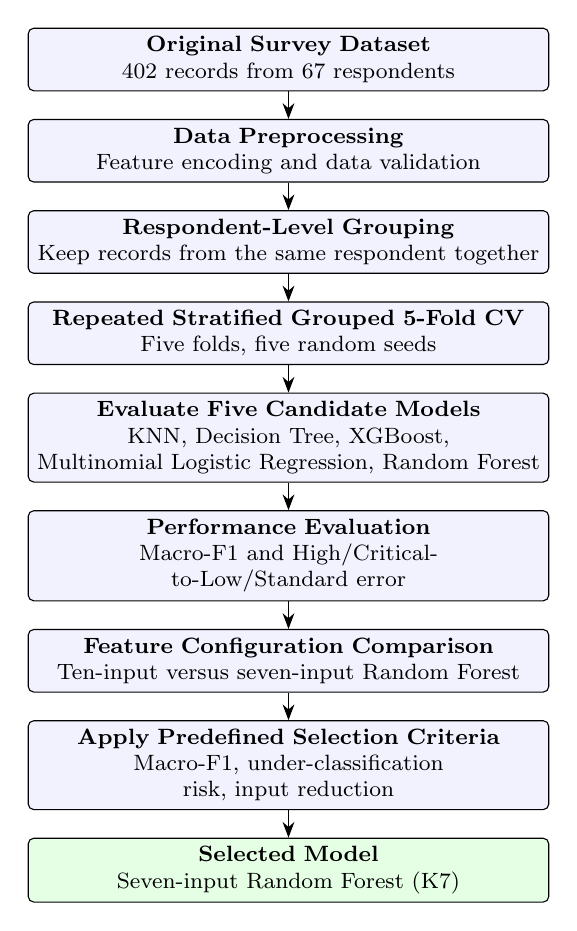
\begin{tikzpicture}[
  stp/.style={draw, fill=blue!5, rounded corners=2pt, align=center, text width=6.4cm, font=\footnotesize,
               inner sep=3pt},
  arr/.style={-{Stealth[length=2mm]}},
  node distance=3.5mm]
\node[stp] (s1) {\textbf{Original Survey Dataset}\\ 402 records from 67 respondents};
\node[stp, below=of s1] (s2) {\textbf{Data Preprocessing}\\ Feature encoding and data validation};
\node[stp, below=of s2] (s3) {\textbf{Respondent-Level Grouping}\\ Keep records from the same
  respondent together};
\node[stp, below=of s3] (s4) {\textbf{Repeated Stratified Grouped 5-Fold CV}\\ Five folds, five
  random seeds};
\node[stp, below=of s4] (s5) {\textbf{Evaluate Five Candidate Models}\\ KNN, Decision Tree,
  XGBoost,\\ Multinomial Logistic Regression, Random Forest};
\node[stp, below=of s5] (s6) {\textbf{Performance Evaluation}\\ Macro-F1 and High/Critical-\\
  to-Low/Standard error};
\node[stp, below=of s6] (s7) {\textbf{Feature Configuration Comparison}\\ Ten-input versus
  seven-input Random Forest};
\node[stp, below=of s7] (s8) {\textbf{Apply Predefined Selection Criteria}\\ Macro-F1,
  under-classification\\ risk, input reduction};
\node[stp, below=of s8, fill=green!10] (s9) {\textbf{Selected Model}\\ Seven-input Random Forest (K7)};
\foreach \a/\b in {s1/s2, s2/s3, s3/s4, s4/s5, s5/s6, s6/s7, s7/s8, s8/s9}
  \draw[arr] (\a) -- (\b);
\end{tikzpicture}
\caption{Experimental methodology for model evaluation and feature selection.}\label{fig2}
\end{figure}

Figure~\ref{fig2} shows how the final Random Forest model was selected, including model
evaluation, respondent-level grouping, feature comparison and selection.

\subsection{Prediction of Security Level}

The security level required for each document is predicted by the selected Random Forest model
from the seven answers given for that document. The prediction does not depend on the vault type;
the vault type decides which final levels are allowed. The personal vault has three levels of
security and the enterprise vault has five. Based on the final level, the encryption algorithm is
selected, so the protection applied always corresponds to the level recorded for the document.

\subsection{Selection of Encryption Configuration}

The encryption configuration is selected from the security level assigned to the document
\cite{sasikumar2025enhancing}. The personal and enterprise vaults use their own hierarchies, so a
personal vault can never hold a High or Critical file. One fixed mapping from level to algorithm
is maintained for both vaults (Table~\ref{tab4}); the vault type only restricts which levels can
be chosen. Both rules are checked again by the storage service, not only by the user interface,
so an incorrect level cannot be stored even if the interface is bypassed.

\subsection{Tokenized Key Management}

The encrypted document and its encryption key are kept apart in DEDV
\cite{rana2023comprehensive}. Every file gets its own randomly generated key. The key material is
serialised, sealed with AES-256-GCM under the vault master key and stored in \code{keys.db}, in a
row found by a random 128-bit token. The token, the file identifier, the algorithm and the level
are bound to the sealed record as additional authenticated data, so a record copied to another
file, or a changed algorithm or level, is detected when the record is opened. The file's row in
\code{vault.db} holds only the token. The token is a reference, not a key: knowing it does not
help without the vault master key, which exists only while the vault is unlocked.

\subsection{Document Retrieval and Decryption}

When a document is requested, the application calls \code{release\_key} with the file's token, the
file identifier and the purpose of the request. The function refuses if the vault is locked, if no
record exists for the token, or if the record belongs to a different file. Otherwise it unseals
the record with the vault master key. Either way it writes an audit entry. The released key is
used to decrypt the file in memory. Every read, re-encryption and self-test goes through this
function; there is no other path to a file key.

\section{System Implementation}\label{sec6}

This section describes the prototype as built: a desktop application for Windows written in
Python. It runs entirely on the user's computer and makes no network connections.

\subsection{Architecture}

The application has three layers (Fig.~\ref{fig3}a). The user interface (PySide6/Qt) has five
pages: View, Upload, Edit, Settings and Developer. It never touches keys or files directly but
calls a service layer: \code{VaultService} (store, read, re-encrypt), \code{SecurityDecisionEngine}
(prediction and vault rules), \code{AuthSession} (password, lock and unlock),
\code{KeyManagementService} (key records and \code{release\_key}), \code{AuditLog} and the
migration service. The services use the cryptographic primitives of the \code{cryptography}
library (OpenSSL), Argon2id from \code{argon2-cffi}, and SQLite for storage.

A vault is a folder with three parts: \code{encrypted\_files} (one ciphertext file per document),
\code{metadata/vault.db} (file metadata and the audit log) and \code{config/keys.db} (the wrapped
vault master key and the per-file key records). The two databases are separate files, so key
material is stored apart from document metadata, but they are opened as one SQLite connection so
that a change that touches both is one transaction. An operating-system file lock ensures that only
one DEDV process opens a vault at a time.

\subsection{Level to Encryption Mapping}

Table~\ref{tab4} gives the mapping from final level to algorithm. Every file uses a new random
key and a random 96-bit nonce; the 128-bit authentication tag of GCM or Poly1305 detects any
change to the ciphertext. For the Enhanced level, the file key is additionally wrapped with
RSA-4096-OAEP under a per-file RSA key pair \cite{rfc8017}. For the Critical level, the file key
is derived with HKDF-SHA256 \cite{rfc5869} from a shared secret encapsulated with ML-KEM-1024, the
lattice-based key-encapsulation mechanism standardised in FIPS 203 \cite{fips203}. In both cases
the private key is stored in the same sealed key record as the rest of the key material, so the
asymmetric step does not add protection beyond the seal under the vault master key; it implements
the configuration that the level names. The Critical level is not claimed to make a file
resistant to quantum computers.

\begin{table}[h]
\caption{Security level to encryption mapping. Personal vaults offer the first three levels;
enterprise vaults offer all five.}\label{tab4}
\begin{tabular}{@{}llll>{\raggedright\arraybackslash}p{4.4cm}@{}}
\toprule
Level & Personal & Enterprise & File encryption & Key material per file \\
\midrule
Low & yes & yes & AES-128-GCM \cite{nist80038d} & 128-bit key \\
Standard & yes & yes & AES-256-GCM & 256-bit key \\
Enhanced & yes & yes & AES-256-GCM & 256-bit key wrapped with RSA-4096-OAEP (SHA-256); RSA
  private key \\
High & no & yes & ChaCha20-Poly1305 \cite{rfc8439} & 256-bit key \\
Critical & no & yes & AES-256-GCM & key from ML-KEM-1024 via HKDF-SHA256; 64-byte ML-KEM
  seed \\
\botrule
\end{tabular}
\end{table}

\subsection{Key Hierarchy}

Fig.~\ref{fig3}b shows the key hierarchy. When a vault is created, the application generates a
random 256-bit vault master key (VMK). The VMK is wrapped twice with AES-256-GCM: once under a key
derived from the vault password with Argon2id \cite{rfc9106} and once under a random 256-bit
recovery key. The Argon2id parameters (time cost 6, memory 256~MiB, parallelism 4) and a random
128-bit salt are stored with the wrapped key; on the test machine one derivation takes about 0.4~s
(Section~\ref{sec8-3}). The password must have at least 12 characters. The recovery key is shown
once, as 13 groups of four Base32 characters, and is never stored. Changing the password, or
resetting it with the recovery key, re-wraps only the VMK; no file is re-encrypted.

The VMK seals every per-file key record (Section~\ref{sec5}). While the vault is unlocked the VMK
is held in memory in a mutable buffer that is overwritten with zeros when the vault locks; in
Python this is a best effort, because the runtime may keep other copies.

\begin{figure}[h]
\centering
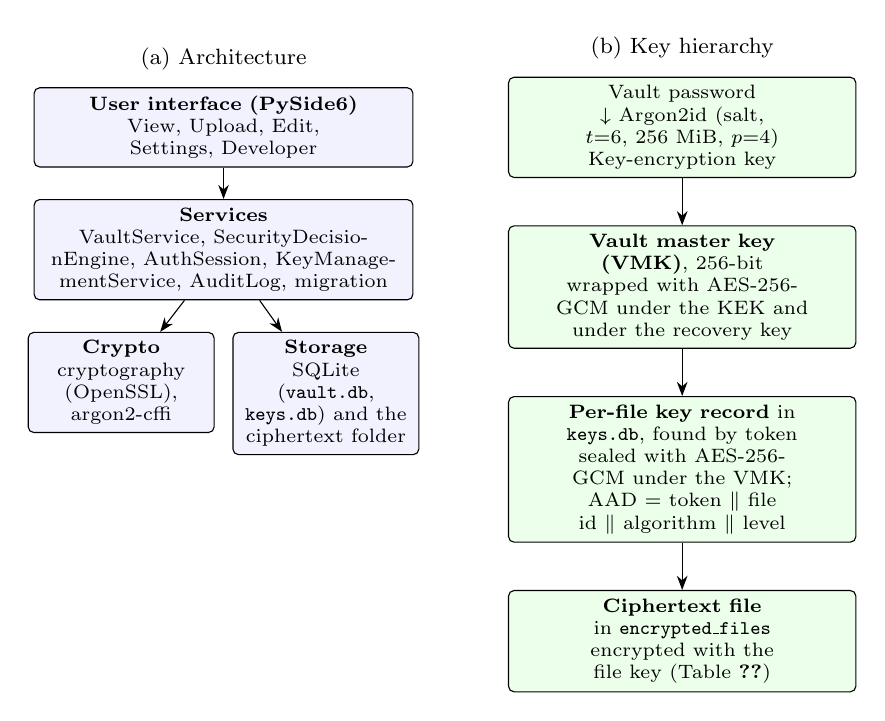
\begin{tikzpicture}[
  lay/.style={draw, fill=blue!5, rounded corners=2pt, align=center, text width=4.6cm,
              font=\scriptsize, inner sep=3pt},
  kb/.style={draw, fill=green!8, rounded corners=2pt, align=center, text width=4.2cm,
             font=\scriptsize, inner sep=3pt},
  arr/.style={-{Stealth[length=1.8mm]}},
  node distance=4mm]
\node[lay] (ui) {\textbf{User interface (PySide6)}\\ View, Upload, Edit, Settings, Developer};
\node[lay, below=of ui] (svc) {\textbf{Services}\\ VaultService, SecurityDecisionEngine,
  AuthSession, KeyManagementService, AuditLog, migration};
\node[lay, below=of svc, text width=2.15cm, xshift=-1.3cm] (cry) {\textbf{Crypto}\\
  cryptography (OpenSSL), argon2-cffi};
\node[lay, below=of svc, text width=2.15cm, xshift=1.3cm] (sto) {\textbf{Storage}\\ SQLite
  (\code{vault.db}, \code{keys.db}) and the ciphertext folder};
\draw[arr] (ui) -- (svc);
\draw[arr] (svc) -- (cry);
\draw[arr] (svc) -- (sto);
\node[font=\footnotesize, above=1mm of ui] {(a) Architecture};

\node[kb, right=12mm of ui] (pw) {Vault password\\ $\downarrow$ Argon2id (salt, $t$=6, 256 MiB,
  $p$=4)\\ Key-encryption key};
\node[kb, below=6mm of pw] (vmk) {\textbf{Vault master key (VMK)}, 256-bit\\ wrapped with
  AES-256-GCM under the KEK and under the recovery key};
\node[kb, below=6mm of vmk] (rec) {\textbf{Per-file key record} in \code{keys.db}, found by
  token\\ sealed with AES-256-GCM under the VMK;\\ AAD = token $\Vert$ file id $\Vert$ algorithm
  $\Vert$ level};
\node[kb, below=6mm of rec] (file) {\textbf{Ciphertext file} in \code{encrypted\_files}\\
  encrypted with the file key (Table~\ref{tab4})};
\draw[arr] (pw) -- (vmk);
\draw[arr] (vmk) -- (rec);
\draw[arr] (rec) -- (file);
\node[font=\footnotesize, above=1mm of pw] {(b) Key hierarchy};
\end{tikzpicture}
\caption{(a) Layers of the implementation. (b) Key hierarchy: the password protects the vault
master key, which protects one key record per file.}\label{fig3}
\end{figure}

\subsection{Authorization and Key Release}

DEDV has one user per vault, and authorization means holding the unlocked vault: the session is
unlocked only after the correct password or recovery key has been given. \code{release\_key}
(Section~\ref{sec5}) is the only function that returns a file key. After three wrong passwords
each further attempt is delayed, starting at 2~s and doubling up to 5~minutes; no data is ever
deleted because of failed attempts. The vault locks itself after a period without keyboard or
mouse activity (10 minutes by default) and on the Lock button: the VMK is erased from memory, every
window that shows vault content is closed and the password is asked again.

\subsection{Audit Log}

Every unlock (successful or failed), lock, store, read, external open, re-encryption, key release,
password creation and change, recovery-key use and migration is written to an \code{audit\_log} table with the
UTC time, the action, the file identifier, the level, the result and a short detail. File
contents, keys and passwords are never logged. The rows form a hash chain: each row stores
SHA-256 of the previous row's hash and its own content, and a ``Verify audit log'' button checks
the whole chain. The chain detects a changed, inserted or deleted row. It is not keyed, so a person
who can write \code{vault.db} could rebuild the whole chain; it does not replace an external,
append-only log.

\subsection{Decision Flow and Upward-Only Override}

After prediction the Upload page shows the predicted class, the confidence and the probability of
every class. The user may choose a higher final level than the prediction, within the levels of
the vault, but never a lower one; for a High/Critical prediction the lowest allowed level is High.
Lower levels are shown disabled with an explanation. If the confidence is below 0.70, or the
prediction is Enhanced (the unreliable class, Section~\ref{sec9}), the user must tick an
acknowledgement before the file can be encrypted. With the shipped model only High/Critical
predictions reach a confidence of 0.70 for any combination of answers, so in practice every Low,
Standard or Enhanced prediction requires this acknowledgement. The Edit page can re-encrypt a
stored file at another level under the same rule: never below the stored prediction. All of these
rules are enforced again in \code{VaultService}, so the interface cannot bypass them. For every
file the vault stores the seven inputs, the predicted class, the confidence, the final level, an
override flag and the time of the decision; the View page shows them.

\subsection{Migration from the First Prototype}

The first prototype (version 0.1) stored metadata in JSON files and wrapped the file keys under a
key kept in a plaintext file. On the first start, version 0.2 converts such a vault: it copies the
old metadata to a backup folder, builds the new databases under temporary names, re-wraps every
file key under a new VMK protected by the password the user chooses, decrypts every file through
the new path to verify it, and only then switches to the new databases. A failure at any step
leaves the old vault unchanged. Ciphertext files are never rewritten. Because the old key file is
shared by all old vaults of a Windows user, it is deleted only after the user confirms.

\subsection{Technology Stack}

Python 3.13, PySide6 6.12 (Qt), \code{cryptography} 50 with OpenSSL 4.0, \code{argon2-cffi} 25.1,
scikit-learn 1.6.1 (the version the model was trained with), SQLite in write-ahead-log mode and
PyInstaller for packaging. The prototype was developed and measured on Windows 11.

\section{Experimentation}\label{sec7}

The experimentation was carried out to evaluate the machine learning models used for
security-level prediction in DEDV and to measure the cost of each security level in the
implementation. The main aim was to compare the five models and identify which one gives the best
result for the classification task.

\subsection{Experimental Setup}

Five machine learning models are used for the experiments: K-Nearest Neighbors (KNN), Random
Forest (RF), XGBoost (XGB), Multinomial Logistic Regression (MLR) and Decision Tree (DT). They are
evaluated on the same prediction task. Only the 402 original records are scored, with
respondent-grouped, stratified five-fold cross-validation repeated with five random seeds
(Fig.~\ref{fig2}); metrics are reported as mean $\pm$ standard deviation over the repeats.

The dataset contains document-related and contextual parameters used to determine the required
security level. These parameters provide the information needed by the models to make their
predictions. The experimental setup focuses on classification performance and the use of the
predicted level in the DEDV workflow.

\subsection{Comparison of Machine Learning Models}

To predict the security level suitable for the document, five models were compared
\cite{theng2024feature}. Each model uses its own method to classify the input data, and the
results provided a basis for selecting the final model. The best macro-F1 was achieved by the
Random Forest model (RF); the other four models are used for comparison.

\subsection{Security-Level Assignment}

After comparison and selection of Random Forest for security level prediction, the seven answers
given for the document are used as inputs for the prediction. The vault environment then decides
which final levels are allowed (Section~\ref{sec4}), and the final level selects the encryption
algorithm (Table~\ref{tab4}).

\subsection{Encryption and Key Management}

Once a security level has been assigned, the algorithm of that level is used to encrypt the
document with a new random key. The ciphertext and the key are stored separately: the ciphertext
in \code{encrypted\_files}, the key in a record of \code{keys.db} sealed under the VMK and found by
a random token. The token is only a reference to the key record and does not contain the key. At
retrieval, \code{release\_key} uses the token to find the record, checks that it belongs to the
requested file and unseals it only for an unlocked session (Section~\ref{sec6}).

\subsection{Experimental Evaluation}\label{sec7-5}

The five models were evaluated by macro-F1 (the primary metric, because the classes are
imbalanced), accuracy and the rate at which High/Critical records are predicted as Low or
Standard. The predicted level is then linked to the corresponding encryption configuration for the
relevant vault.

The cost of every security level was measured with a benchmark script that is part of the
implementation (\code{bench/benchmark.py}). For each of the five levels and for files of 1~KB,
100~KB, 1~MB, 10~MB and 50~MB (seeded random data) it measures: (i) the encryption primitive
alone, including the per-file key generation the level requires, and the matching decryption;
(ii) end-to-end storing and reading through the vault service, which includes reading and writing
the files, sealing or unsealing the key record, the database transaction and the audit entries;
(iii) the storage overhead of the ciphertext file and of the key record; and (iv) the peak Python
heap during each operation. It also measures one prediction of the model and one unlock with the
stored Argon2id parameters. Each measurement uses two warm-up runs and 20 timed repetitions,
reported as median and interquartile range (IQR); the five levels are interleaved in a rotating
order in every repetition. DEDV loads whole files into memory, so the file sizes stop at 50~MB on
purpose. The test machine was an AMD Ryzen~7 7840HS laptop (16 logical CPUs, 16~GB RAM) with
Windows 11, Python 3.13 and OpenSSL 4.0.

The results are discussed in the next section.

\section{Results and Discussion}\label{sec8}

Five machine learning models were tested on the experimental data for predicting the security
level of documents. Among the models, Random Forest yielded the highest macro-F1 score among the
main configurations and was selected for further evaluation. The input selection produced a
seven-input Random Forest with a macro-F1 score of 0.380~$\pm$~0.024 and an accuracy of 72.5\%.

\subsection{Model Comparison}\label{sec8-1}

Random Forest with ten inputs yielded a macro-F1 score of 0.389, while the seven-input model
achieved 0.380. The small difference suggests that the smaller input model retains similar overall
classification performance under the selected evaluation procedure \cite{theng2024feature}.

% VERIFY: CONTEXT_PROMPT.md confirms only the macro-F1 means of MLR (0.345), XGB (0.334),
% DT (0.324) and RF-10 (0.389 +/- 0.026). The KNN row, the +/- values of DT, XGB and MLR, and
% every accuracy value in this table are copied from the original paper and were not verified.
\begin{table}[h]
\caption{Comparison of Candidate Machine Learning Models}\label{tab2}
\begin{tabular}{@{}lcc@{}}
\toprule
Model & Macro-F1 & Accuracy (\%) \\
\midrule
K-Nearest Neighbors (KNN) & 0.320 $\pm$ 0.019 & 75.0 $\pm$ 0.6 \\
Decision Tree (DT) & 0.324 $\pm$ 0.033 & 59.6 $\pm$ 1.4 \\
XGBoost (XGB) & 0.334 $\pm$ 0.021 & 69.5 $\pm$ 0.3 \\
Multinomial Logistic Regression (MLR) & 0.345 $\pm$ 0.013 & 77.0 $\pm$ 0.8 \\
Random Forest (10 inputs) & 0.389 $\pm$ 0.026 & 75.4 $\pm$ 0.8 \\
\botrule
\end{tabular}
\end{table}

Random Forest achieved the highest macro-F1 among the five candidate models, whereas Multinomial
Logistic Regression achieved the highest reported accuracy. Accuracy is not a useful selection
metric here: always predicting the majority class (High/Critical) already reaches 75.4\% accuracy
with a macro-F1 of only 0.215. Random Forest was therefore selected based on macro-F1 and the
additional under-classification and feature-reduction criteria, rather than accuracy alone.

The selection criteria were fixed before the runs, with the ten-input Random Forest as reference.
A configuration was adequate if its macro-F1 was at least the reference minus one standard
deviation (0.364) and its High/Critical-to-Low/Standard error rate was at most the reference
(13.0\%) plus three percentage points (16.0\%). Among adequate configurations the one with the
fewest inputs was chosen. The seven-input model has a slightly lower macro-F1 than the ten-input
model, and its High/Critical-to-Low/Standard error rate is 15.9\%, compared with 13.0\% for the
ten-input model (Table~\ref{tab3}).

The results show a trade-off between classification performance and the number of inputs. The
seven-input model met the predefined selection criteria while requiring fewer inputs than the
ten-input model, hence it was selected. It retains most of the overall performance of the
reference model even though its macro-F1 is slightly lower (0.380 compared to 0.389). The
reduction in inputs costs a small loss in macro-F1 and a higher risk of under-classification; its
error rate passes the 16.0\% limit by only 0.1 percentage point.

% VERIFY: the accuracy of the ten-input RF (75.4 +/- 0.8) and the +/- 1.6 of the seven-input RF
% are not in CONTEXT_PROMPT.md; 72.5 % (seven-input accuracy) is.
\begin{table}[h]
\caption{Comparison of Ten-Input and Seven-Input Random Forest Models}\label{tab3}
\begin{tabular}{@{}lcc@{}}
\toprule
Metric & 10-Input RF & 7-Input RF (K7) \\
\midrule
Macro-F1 & 0.389 $\pm$ 0.026 & 0.380 $\pm$ 0.024 \\
Accuracy (\%) & 75.4 $\pm$ 0.8 & 72.5 $\pm$ 1.6 \\
Number of input features & 10 & 7 \\
High/Critical $\rightarrow$ Low/Standard error (\%) & 13.0 & 15.9 \\
\botrule
\end{tabular}
\end{table}

\subsection{Implications for DEDV}

The results support Random Forest as a decision support component for assigning a security level
to a document. The seven selected attributes capture information about document sensitivity, usage
patterns, access requirements, exposure consequences and protection duration. This way DEDV
follows a context-aware approach without relying on the scenario identifier as one of the inputs.
The Enhanced class is not reliably classified in the current results \cite{park2022majority}.
Further validation using a more representative data set is required for reliable security-critical
decision making. For this reason the implementation shows the confidence of every prediction, asks
for an acknowledgement when the prediction is uncertain or Enhanced, and lets the user raise but
never lower the level (Section~\ref{sec6}). Classification performance alone does not establish
the cost of the encryption; Section~\ref{sec8-3} reports it.

\subsection{Encryption Performance}\label{sec8-3}

Table~\ref{tab5} and Figs.~\ref{fig4}--\ref{fig5} summarise the measurements described in
Section~\ref{sec7-5}. All times are medians of 20 repetitions; the IQR is given in parentheses. The
complete data are in \code{bench/results} of the implementation.

\begin{table}[h]
\caption{Storage overhead per file, end-to-end store and read times in ms (median, IQR in
parentheses) and primitive encryption throughput at 50~MB.}\label{tab5}
\begin{tabular}{@{}lrrrrrr@{}}
\toprule
 & Overhead & \multicolumn{2}{c}{1 MB file} & \multicolumn{2}{c}{50 MB file} & Encrypt \\
\cmidrule(lr){3-4}\cmidrule(lr){5-6}
Level & (bytes) & Store & Read & Store & Read & (MB/s) \\
\midrule
Low & 118 & 6.6 (1.1) & 12.2 (1.6) & 97.7 (6.2) & 47.3 (2.5) & 2{,}507 \\
Standard & 138 & 6.1 (1.4) & 11.7 (1.4) & 99.8 (7.9) & 47.6 (4.7) & 2{,}415 \\
Enhanced & 3{,}975 & 461 (439) & 293 (20) & 842 (478) & 328 (6) & 142 \\
High & 138 & 7.3 (1.2) & 12.6 (2.0) & 118 (17) & 60.4 (3.2) & 1{,}530 \\
Critical & 2{,}301 & 7.7 (1.1) & 12.3 (2.4) & 103 (7) & 49.2 (2.9) & 2{,}401 \\
\botrule
\end{tabular}
\end{table}

Four of the five levels cost about the same. At Low, Standard, High and Critical, storing a 1~MB
file took 6.1--7.7~ms and reading it 11.7--12.6~ms, although the cryptographic operations alone
took only 1.0--1.5~ms (encryption) and 1.2--1.8~ms (decryption). Most of the end-to-end time is
spent outside the cipher: the database transaction with its synchronous commit, and for a read
two audit commits (key release and read) and the first opening of a newly written file, which the
operating system's antivirus scanner inspects (about 8~ms on the test machine). For 50~MB files,
storing took 98--118~ms and reading 47--60~ms. ChaCha20-Poly1305 (High) was somewhat slower than
AES-GCM on this processor, which has hardware AES instructions. ML-KEM-1024 (Critical) added about
0.5~ms per file for key generation and encapsulation.

The Enhanced level is the exception. Every file gets a new RSA-4096 key pair, and generating it
took 0.29--0.55~s (median of the primitive encryption at each size) with a wide IQR, because key generation searches
for random primes; storing a file took 0.37--0.84~s. Reading took about 0.3~s at every size, almost
all of it spent loading the RSA private key, which the cryptographic library validates on every
load (about 0.28~s on the test machine), not in the RSA decryption itself (about 2~ms).

\begin{figure}[h]
\centering
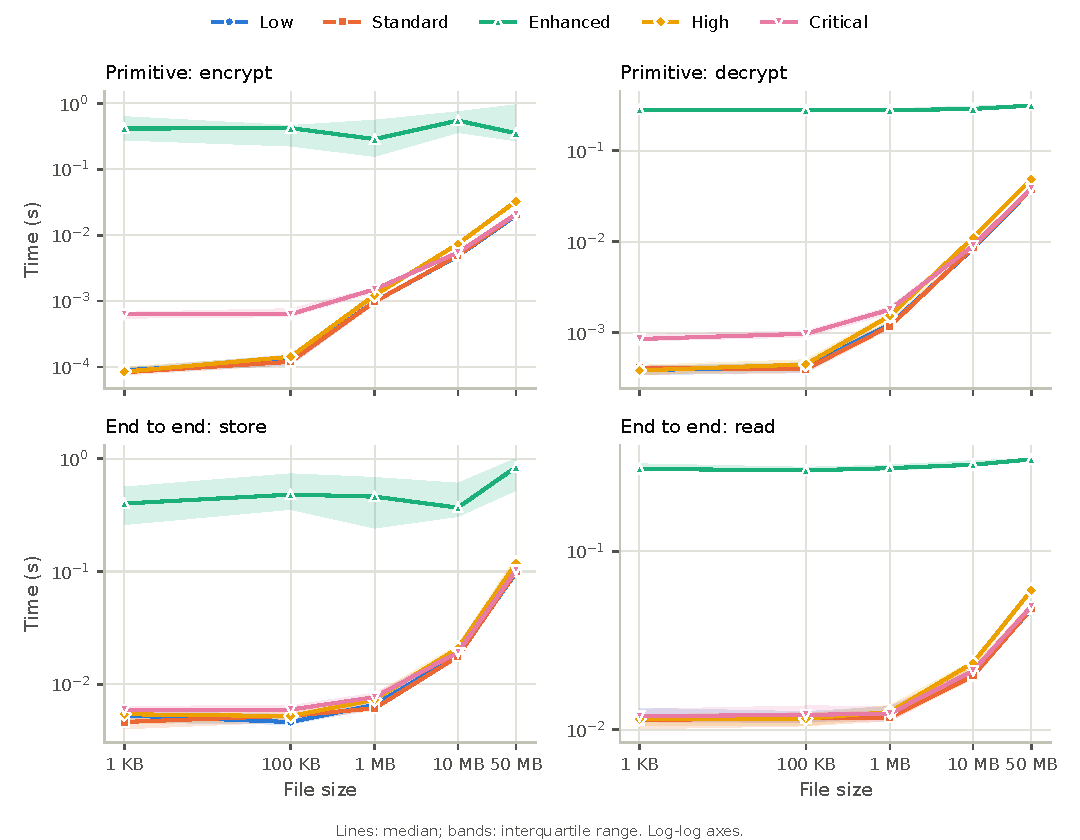
\includegraphics[width=\textwidth]{time_vs_size.pdf}
\caption{Time versus file size for each security level (log-log): primitive encryption and
decryption (top) and end-to-end store and read through the vault service (bottom). Lines are
medians of 20 repetitions; bands are interquartile ranges.}\label{fig4}
\end{figure}

\begin{figure}[h]
\centering
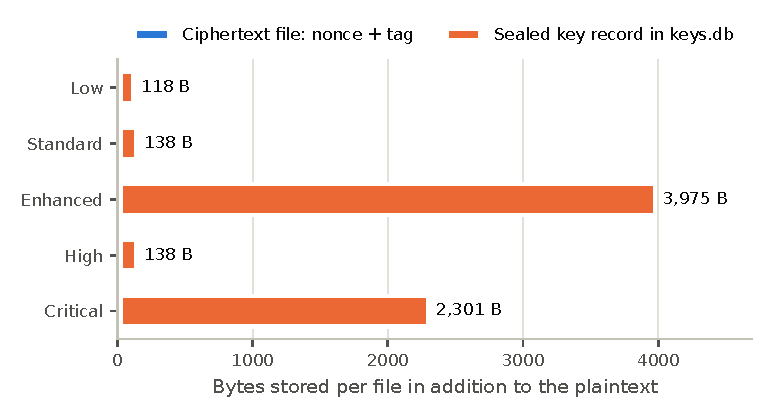
\includegraphics[width=0.8\textwidth]{overhead.pdf}
\caption{Bytes stored per file in addition to the plaintext: ciphertext-file overhead (nonce and
tag, 28 bytes at every level) and the sealed key record in \code{keys.db}.}\label{fig5}
\end{figure}

Every ciphertext file is exactly 28 bytes larger than the plaintext (12-byte nonce and 16-byte
tag) at every level (Fig.~\ref{fig5}). The sealed key record adds 90 bytes at Low, 110 bytes at
Standard and High, 2,273 bytes at Critical (ML-KEM ciphertext and seed) and 3,947 bytes at Enhanced
(RSA private key and wrapped key). For a 1~MB file this is below 0.4\% at every level; for a 1~KB
file the Enhanced overhead is almost four times the file size. The peak Python heap was about twice
the file size for encryption and three times for decryption and for storing, because the plaintext
and the ciphertext are held in memory at the same time; this is why the measured sizes stop at
50~MB. Unlocking the vault (Argon2id with 256~MiB of memory) took 0.41~s (IQR 0.007~s), once per
session, and one prediction of the model took 18~ms.

\section{Limitations}\label{sec9}

The limitations concern the prediction model and the prototype.

\textbf{Prediction model.} First, the original data contain 402 records, and only eight of them
belong to the Enhanced class, so the classification results are not reliable for that class. The
precision and recall of the seven-input Random Forest for Enhanced are both approximately 0.10.
Because of the limited number of responses, the model could not learn consistent patterns for the
Enhanced class, which also makes the evaluation metrics less reliable. Hence the overall macro-F1
should not be read as equally strong performance across all four security levels. An additional
survey with representative data and a review of the rules used to assign the target labels are
necessary to improve the reliability of this class. Second, the seven-input model reduced the
number of required inputs from ten to seven while retaining a macro-F1 close to that of the
ten-input model, but its High/Critical-to-Low/Standard error rate increased from 13.0\% to 15.9\%,
just inside the predefined limit of 16.0\%; this remains important for security-sensitive use.
Third, the model has been evaluated on survey data only and has not yet been verified in
real-world use.

Figure~\ref{fig6} shows a confusion matrix from a related experiment, in which the Random Forest
was trained on the respondents' own survey answer as the target label. In that labelling 178
records are Enhanced, so the matrix illustrates how hard Enhanced is to separate from the
neighbouring levels, but it is not the confusion matrix of the selected K7 model, which uses a
target with eight Enhanced records. The K7 confusion matrix is not available in this work.

\textbf{Prototype.} The vault has a single user: there are no accounts or roles, and the Personal
or Enterprise type is a setting of the application, not an access-control mechanism. Keys are
protected by the password only; there is no hardware-backed key storage such as a TPM. The VMK is
erased from memory on lock, and temporary plaintext copies opened in other programs are
overwritten before deletion, but both are best effort: Python may keep other copies in memory, and
on solid-state drives, journaling file systems or with backup tools an overwrite does not
guarantee that the old data are gone. The audit chain is not keyed (Section~\ref{sec6}). DEDV
loads whole files into memory, which limits the practical file size. The installer is not
code-signed.

% VERIFY: Fig. 6 is redrawn from the counts printed in the original PDF (rows 20 / 71 / 178 / 133,
% i.e. the survey-answer target). The K7 model's confusion matrix is not in this repository or in
% CONTEXT_PROMPT.md; replace this figure if it becomes available.
\begin{figure}[h]
\centering
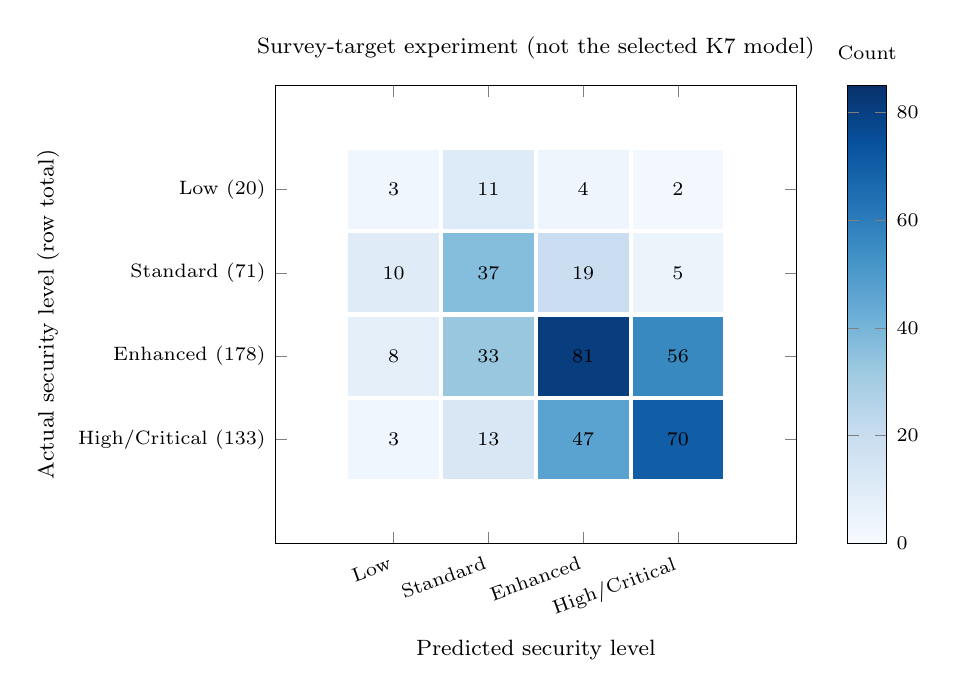
\begin{tikzpicture}
\begin{axis}[
  title={Survey-target experiment (not the selected K7 model)},
  title style={font=\footnotesize},
  width=8.2cm, height=7.4cm,
  enlargelimits={abs=0.75}, axis on top,
  colormap/Blues, colorbar,
  colorbar style={title={Count}, title style={font=\scriptsize}, tick label style={font=\scriptsize}},
  point meta min=0, point meta max=85,
  xtick={0,1,2,3}, ytick={0,1,2,3},
  xticklabels={Low,Standard,Enhanced,High/Critical},
  yticklabels={Low (20),Standard (71),Enhanced (178),High/Critical (133)},
  x tick label style={rotate=20, anchor=north east, font=\scriptsize},
  y tick label style={font=\scriptsize},
  xlabel={Predicted security level}, ylabel={Actual security level (row total)},
  label style={font=\footnotesize},
  y dir=reverse,
  nodes near coords, nodes near coords style={font=\scriptsize, anchor=center},
]
\addplot[matrix plot*, mesh/cols=4, point meta=explicit, draw=white, line width=1.5pt] table[meta=c] {
x y c
0 0 3
1 0 11
2 0 4
3 0 2
0 1 10
1 1 37
2 1 19
3 1 5
0 2 8
1 2 33
2 2 81
3 2 56
0 3 3
1 3 13
2 3 47
3 3 70
};
\end{axis}
\end{tikzpicture}
\caption{Confusion matrix of a Random Forest trained with the respondents' survey answer as the
target (402 records, 178 of them Enhanced). It is shown to illustrate the difficulty of the
Enhanced class and is not the confusion matrix of the selected seven-input model (K7), whose
target has eight Enhanced records. Values are prediction counts.}\label{fig6}
\end{figure}

\section{Future Scope of Work}\label{sec10}

The prediction model should be trained on a larger and more diverse dataset, with many more
Enhanced examples from different respondents, and validated in real-world scenarios with real
documents. The prototype could add hardware-backed key protection (for example the operating
system's key store or a TPM), several users with roles, an audit log protected by a key or by an
external append-only store, streaming encryption so that large files need not fit in memory, and
a code-signed installer. A user study could test whether the confidence display and the
acknowledgement step lead to better level choices.

\section{Conclusion}\label{sec11}

This paper presents the Dynamic Encryption Digital Vault (DEDV), a framework and working prototype
for document storage. The system assigns a document a security level based on contextual
attributes such as sensitivity, usage patterns, access requirements and exposure consequences.
Random Forest achieved the best macro-F1 among the evaluated models: 0.389 with ten inputs and
0.380 with the selected seven-input configuration. The prototype maps every level to a defined
encryption algorithm, protects all file keys with a password-derived key hierarchy, keeps them in a
separate token-indexed key store, releases them only to an unlocked session and records every
release in a hash-chained audit log. Measurements on a laptop show that four of the five levels
store or read a 1~MB file in about 6--13~ms, mostly spent on database commits rather than on
encryption, while the Enhanced level costs 0.3--0.8~s per file because of its per-file RSA-4096 key
pair. The limited number of Enhanced records
affects classification reliability; the effectiveness of the system will improve with better data
and real-world validation.

\bibliography{DEDV_2_revised}

\end{document}
